\documentclass[10pt,a4paper]{article}
\usepackage[utf8]{inputenc}
\usepackage[spanish,es-tabla]{babel}
\usepackage{geometry}
\geometry{top=2.0cm, bottom=2.0cm, left=2.0cm, right=2.0cm}
\usepackage{amsmath,amssymb,amsfonts}
\usepackage{graphicx}
\usepackage{booktabs}
\usepackage{array}
\usepackage{xcolor}
\usepackage{tikz}
\usepackage{circuitikz}
\usepackage{fancyhdr}
\usepackage{titlesec}
\usepackage{colortbl}
\usepackage{hyperref}
\usepackage{float}
\usepackage{siunitx}
\usepackage{subcaption}

% Colores institucionales sobrios
\definecolor{colorprimario}{RGB}{24, 76, 120}     % Azul institucional LSD
\definecolor{colorsecundario}{RGB}{70, 90, 120}   % Gris azulado
\definecolor{colorfondo}{RGB}{245, 247, 250}      % Gris muy claro
\definecolor{colorlinea}{RGB}{200, 210, 220}

\hypersetup{
    hypertexnames=false,
    colorlinks=true,
    linkcolor=colorprimario,
    citecolor=colorprimario,
    urlcolor=colorprimario
}

\pagestyle{fancy}
\fancyhf{}
\fancyhead[L]{\small\bfseries\color{colorprimario} Laboratorio de Sistemas Dinámicos}
\fancyhead[R]{\small\color{colorsecundario} Front-End sEMG AD620 \textbar{} Rev. 1.0}
\fancyfoot[L]{\small\color{colorsecundario} S. Prado Rodríguez -- L. G. Braunstein}
\fancyfoot[R]{\small\color{colorsecundario} Página \thepage}
\renewcommand{\headrulewidth}{0.6pt}
\renewcommand{\footrulewidth}{0.4pt}

% Formato sobrio de títulos sin paréntesis ni palabras de relleno
\titleformat{\section}{\large\bfseries\color{colorprimario}}{\thesection.}{0.6em}{}[\titlerule]
\titleformat{\subsection}{\normalsize\bfseries\color{colorsecundario}}{\thesubsection.}{0.5em}{}
\titleformat{\subsubsection}{\small\bfseries\color{colorsecundario}}{\thesubsubsection.}{0.4em}{}

\begin{document}

% -------------------------------------------------------------
% ENCABEZADO DE HOJA DE DATOS (DATASHEET)
% -------------------------------------------------------------
\begin{center}
    
\includegraphics[height=2.2cm]{imagenes/logo_nandu_lsd.png}\\[0.5em]
    {\Huge\bfseries\color{colorprimario} HOJA DE DATOS TÉCNICOS}\\[0.3em]
    {\Large\bfseries Amplificador Diferencial de 3 Canales}\\[0.2em]
    {\large Basado en Amplificador de Instrumentación AD620 y Protección Activa por MOSFETs}\\[0.5em]
    \rule{\linewidth}{1.2pt}\\[0.4em]
    {\normalsize\bfseries Autores: Santiago Prado Rodríguez -- Lucas Gastón Braunstein}\\[0.2em]
    {\small\textit{Laboratorio de Sistemas Dinámicos -- Universidad de Buenos Aires}}\\[0.2em]
    {\small Documentación Técnica de Hardware -- Septiembre 2026}
\end{center}

\vspace{0.5em}

% -------------------------------------------------------------
% SECCIÓN 1: ESQUEMA DEL CIRCUITO Y DISEÑO DE PCB
% -------------------------------------------------------------
\section{Esquema del Circuito y Diseño de PCB}

El sistema de adquisición sEMG se organiza en una arquitectura tricanal diferencial de alta simetría. A continuación se presentan el esquema electrónico integral de la placa (Figura \ref{fig:esquema_completo_3canales}) y su trazado físico en circuito impreso (Figura \ref{fig:pcb_layout}), seguidos por el desglose analítico de cada bloque constituyente.

\begin{figure}[H]
\centering
\resizebox{\linewidth}{!}{%
\begin{circuitikz}[american, thick, font=\sffamily]
%
  % ====================================================
  % BLOQUE 1: ALIMENTACION Y PROTECCION ACTIVA (IZQUIERDA)
  % ====================================================
  \begin{scope}[xshift=-14cm, yshift=0cm]
    \draw[dashed, draw=blue!60, fill=blue!2, rounded corners] (-2.8, 9.2) rectangle (13.6, -9.2);
    \node[anchor=north west, font=\bfseries\color{blue!70!black}] at (-2.5, 8.8) {ETAPA DE ALIMENTACI\'ON Y PROTECCI\'ON ACTIVA $\pm 9\,\text{V}$};

    % Bornera BAT TBLOCK-M3
    \draw (-2.2, 5.0) rectangle (0.4, -5.0);
    \node[font=\bfseries] at (-0.9, 4.4) {BAT};
    \node[font=\scriptsize, anchor=west] at (-2.0, 3.4) {Pin 1: +9V};
    \node[font=\scriptsize, anchor=west] at (-2.0, 0.0) {Pin 2: GND};
    \node[font=\scriptsize, anchor=west] at (-2.0, -3.4) {Pin 3: -9V};
    \draw (0.4, 3.4) -- (1.6, 3.4);
    \draw (0.4, 0.0) -- (1.0, 0.0) node[ground]{};
    \draw (0.4, -3.4) -- (1.6, -3.4);

    % Bornera SWITCH TBLOCK-M4
    \draw (1.6, 5.0) rectangle (3.8, -5.0);
    \node[font=\bfseries] at (2.7, 4.4) {SWITCH};
    \node[font=\scriptsize] at (2.0, 3.4) {1}; \node[font=\scriptsize] at (3.4, 3.4) {2};
    \node[font=\scriptsize] at (2.0, -3.4) {3}; \node[font=\scriptsize] at (3.4, -3.4) {4};
    \draw[very thick] (2.2, 3.4) -- (3.2, 3.4);
    \draw[very thick] (2.2, -3.4) -- (3.2, -3.4);

    % Fusibles
    \draw (3.8, 3.4) to[fuse, *-*, l={\small $\text{FUSP} = 0.25\,\text{A}$}] (6.0, 3.4);
    \draw (3.8, -3.4) to[fuse, *-*, l_={\small $\text{FUSN} = 0.25\,\text{A}$}] (6.0, -3.4);

    % --- RIEL POSITIVO (+9V) ---
    \draw (6.0, 3.4) -- (7.2, 3.4) coordinate (s_pos)
          node[pmos, rotate=90, yscale=-1, anchor=S] (QP) {};
    \node[above=6pt, font=\small\bfseries] at (7.2, 3.7) {F9540N};
    \draw (QP.D) -- (12.2, 3.4) node[circle, fill, inner sep=2pt]{} 
          node[right, font=\bfseries\color{red!70!black}] {+9V};

    \draw (QP.G) -- (7.2, 1.8) coordinate (g_pos) -- (9.2, 1.8);
    \draw (8.0, 3.4) to[zD, *-, l_={\small $D_2$}] (8.0, 1.8) node[circ]{};
    \draw (9.2, 1.8) to[R, *-, l={\small $R_3 = 10\,\text{k}\Omega$}] (9.2, 0.0);

    % --- RIEL NEGATIVO (-9V) ---
    \draw (6.0, -3.4) -- (7.2, -3.4) coordinate (s_neg)
          node[nmos, rotate=-90, yscale=-1, anchor=S] (QN) {};
    \node[below=6pt, font=\small\bfseries] at (7.2, -3.7) {IRFZ44N};
    \draw (QN.D) -- (12.2, -3.4) node[circle, fill, inner sep=2pt]{} 
          node[right, font=\bfseries\color{blue!70!black}] {-9V};

    \draw (QN.G) -- (7.2, -1.8) coordinate (g_neg) -- (10.2, -1.8);
    \draw (8.0, -3.4) to[zD, *-, l={\small $D_1$}] (8.0, -1.8) node[circ]{};
    \draw (10.2, -1.8) to[R, *-, l={\small $R_1 = 10\,\text{k}\Omega$}] (10.2, 0.0);

    % Resistencias Bleeder
    \draw (11.2, 3.4) to[R, *-, l_={\small $R_4 = 100\,\text{k}\Omega$}] (11.2, 0.0);
    \draw (11.2, -3.4) to[R, *-, l={\small $R_2 = 100\,\text{k}\Omega$}] (11.2, 0.0);

    % Masa GND
    \draw (6.8, 0.0) node[ground]{} -- (12.2, 0.0) node[circle, fill, inner sep=2pt]{} 
          node[right, font=\bfseries] {GND};
    \draw (9.2, 0.0) node[circ]{};
    \draw (10.2, 0.0) node[circ]{};
    \draw (11.2, 0.0) node[circ]{};
  \end{scope}

  % ====================================================
  % BLOQUE 2: CANAL 1 (U1 - AD620)
  % ====================================================
  \begin{scope}[xshift=4.8cm, yshift=6.0cm]
    \draw[dashed, draw=blue!60, fill=blue!2, rounded corners] (-3.8, 2.8) rectangle (9.6, -2.8);
    \node[anchor=north west, font=\bfseries\color{blue!70!black}] at (-3.5, 2.5) {CANAL 1};

    % Bornera IN1
    \draw (-3.4, 1.3) rectangle (-2.0, -1.3);
    \node[font=\bfseries\scriptsize] at (-2.7, 0.9) {IN1};
    \node[font=\tiny] at (-3.1, 0.45) {1}; \draw (-2.0, 0.45) -- (-1.6, 0.45) node[ground]{};
    \node[font=\tiny] at (-3.1, 0.0) {2};  \draw (-2.0, 0.0) -- (-1.0, 0.0) -- (-1.0, 0.9) coordinate (in1_neg_start);
    \node[font=\tiny] at (-3.1, -0.45) {3}; \draw (-2.0, -0.45) -- (-1.0, -0.45) -- (-1.0, -0.9) coordinate (in1_pos_start);

    % Filtros de entrada
    \draw (in1_neg_start) to[C, l={\scriptsize $C_2 = 33\,\text{nF}$}] (0.8, 0.9) coordinate (junc1_neg) -- (3.0, 0.9);
    \draw (junc1_neg) to[R, *-, l_={\scriptsize $R_2 = 100\,\text{k}\Omega$}] (0.8, 1.7) node[ground, yscale=-1]{};

    \draw (in1_pos_start) to[C, l_={\scriptsize $C_1 = 33\,\text{nF}$}] (0.8, -0.9) coordinate (junc1_pos) -- (3.0, -0.9);
    \draw (junc1_pos) to[R, *-, l={\scriptsize $R_1 = 100\,\text{k}\Omega$}] (0.8, -1.7) node[ground]{};

    % AD620 (U1)
    \draw[thick] (3.0, 1.4) -- (5.4, 0.0) -- (3.0, -1.4) -- cycle;
    \node at (4.1, 0.0) {\small AD620};
    \node[below=4pt, font=\tiny] at (4.1, 0.0) {U1};
    \node at (3.3, 0.9) {\scriptsize \(-\)};
    \node at (3.3, -0.9) {\scriptsize \(+\)};

    % Resistencia de ganancia RG (Pin 1 y 8)
    \draw (3.0, 0.4) node[right=1pt, font=\tiny] {1} -- (2.2, 0.4) coordinate (rg1_top);
    \draw (3.0, -0.4) node[right=1pt, font=\tiny] {8} -- (2.2, -0.4) coordinate (rg1_bot);
    \draw (rg1_top) to[R, *-*, l_={\scriptsize $R_3 = 100\,\Omega$}] (rg1_bot);

    % Alimentación U1
    \draw (3.8, 0.9) -- ++(0, 0.7) node[above, font=\tiny\bfseries\color{red!70!black}] {+9V};
    \draw (3.8, -0.9) -- ++(0, -0.7) node[below, font=\tiny\bfseries\color{blue!70!black}] {-9V};
    \draw (4.6, -0.5) -- ++(0, -0.7) node[ground]{};

    % Salida y Bornera OUT1
    \draw (5.4, 0.0) -- (7.6, 0.0) coordinate (out1_wire);
    \draw (7.6, 1.0) rectangle (9.2, -1.0);
    \node[font=\bfseries\scriptsize] at (8.4, 0.6) {OUT1};
    \node[font=\tiny] at (8.0, 0.0) {2}; \draw (out1_wire) -- (7.6, 0.0);
    \node[font=\tiny] at (8.0, -0.5) {1}; \draw (9.2, -0.5) -- ++(0.3, 0) node[ground]{};
  \end{scope}

  % ====================================================
  % BLOQUE 3: CANAL 2 (U2 - AD620)
  % ====================================================
  \begin{scope}[xshift=4.8cm, yshift=0.0cm]
    \draw[dashed, draw=blue!60, fill=blue!2, rounded corners] (-3.8, 2.8) rectangle (9.6, -2.8);
    \node[anchor=north west, font=\bfseries\color{blue!70!black}] at (-3.5, 2.5) {CANAL 2};

    % Bornera IN2
    \draw (-3.4, 1.3) rectangle (-2.0, -1.3);
    \node[font=\bfseries\scriptsize] at (-2.7, 0.9) {IN2};
    \node[font=\tiny] at (-3.1, 0.45) {1}; \draw (-2.0, 0.45) -- (-1.6, 0.45) node[ground]{};
    \node[font=\tiny] at (-3.1, 0.0) {2};  \draw (-2.0, 0.0) -- (-1.0, 0.0) -- (-1.0, 0.9) coordinate (in2_neg_start);
    \node[font=\tiny] at (-3.1, -0.45) {3}; \draw (-2.0, -0.45) -- (-1.0, -0.45) -- (-1.0, -0.9) coordinate (in2_pos_start);

    % Filtros de entrada
    \draw (in2_neg_start) to[C, l={\scriptsize $C_4 = 33\,\text{nF}$}] (0.8, 0.9) coordinate (junc2_neg) -- (3.0, 0.9);
    \draw (junc2_neg) to[R, *-, l_={\scriptsize $R_4 = 100\,\text{k}\Omega$}] (0.8, 1.7) node[ground, yscale=-1]{};

    \draw (in2_pos_start) to[C, l_={\scriptsize $C_3 = 33\,\text{nF}$}] (0.8, -0.9) coordinate (junc2_pos) -- (3.0, -0.9);
    \draw (junc2_pos) to[R, *-, l={\scriptsize $R_5 = 100\,\text{k}\Omega$}] (0.8, -1.7) node[ground]{};

    % AD620 (U2)
    \draw[thick] (3.0, 1.4) -- (5.4, 0.0) -- (3.0, -1.4) -- cycle;
    \node at (4.1, 0.0) {\small AD620};
    \node[below=4pt, font=\tiny] at (4.1, 0.0) {U2};
    \node at (3.3, 0.9) {\scriptsize \(-\)};
    \node at (3.3, -0.9) {\scriptsize \(+\)};

    % Resistencia de ganancia RG (Pin 1 y 8)
    \draw (3.0, 0.4) node[right=1pt, font=\tiny] {1} -- (2.2, 0.4) coordinate (rg2_top);
    \draw (3.0, -0.4) node[right=1pt, font=\tiny] {8} -- (2.2, -0.4) coordinate (rg2_bot);
    \draw (rg2_top) to[R, *-*, l_={\scriptsize $R_6 = 100\,\Omega$}] (rg2_bot);

    % Alimentación U2
    \draw (3.8, 0.9) -- ++(0, 0.7) node[above, font=\tiny\bfseries\color{red!70!black}] {+9V};
    \draw (3.8, -0.9) -- ++(0, -0.7) node[below, font=\tiny\bfseries\color{blue!70!black}] {-9V};
    \draw (4.6, -0.5) -- ++(0, -0.7) node[ground]{};

    % Salida y Bornera OUT2
    \draw (5.4, 0.0) -- (7.6, 0.0) coordinate (out2_wire);
    \draw (7.6, 1.0) rectangle (9.2, -1.0);
    \node[font=\bfseries\scriptsize] at (8.4, 0.6) {OUT2};
    \node[font=\tiny] at (8.0, 0.0) {2}; \draw (out2_wire) -- (7.6, 0.0);
    \node[font=\tiny] at (8.0, -0.5) {1}; \draw (9.2, -0.5) -- ++(0.3, 0) node[ground]{};
  \end{scope}

  % ====================================================
  % BLOQUE 4: CANAL 3 (U3 - AD620)
  % ====================================================
  \begin{scope}[xshift=4.8cm, yshift=-6.0cm]
    \draw[dashed, draw=blue!60, fill=blue!2, rounded corners] (-3.8, 2.8) rectangle (9.6, -2.8);
    \node[anchor=north west, font=\bfseries\color{blue!70!black}] at (-3.5, 2.5) {CANAL 3};

    % Bornera IN3GND
    \draw (-3.4, 1.3) rectangle (-2.0, -1.3);
    \node[font=\bfseries\scriptsize] at (-2.7, 0.9) {IN3GND};
    \node[font=\tiny] at (-3.1, 0.45) {1}; \draw (-2.0, 0.45) -- (-1.4, 0.45) node[ground]{} node[right=2pt, font=\tiny\bfseries] {REF};
    \node[font=\tiny] at (-3.1, 0.0) {2};  \draw (-2.0, 0.0) -- (-1.0, 0.0) -- (-1.0, 0.9) coordinate (in3_neg_start);
    \node[font=\tiny] at (-3.1, -0.45) {3}; \draw (-2.0, -0.45) -- (-1.0, -0.45) -- (-1.0, -0.9) coordinate (in3_pos_start);

    % Filtros de entrada
    \draw (in3_neg_start) to[C, l={\scriptsize $C_6 = 33\,\text{nF}$}] (0.8, 0.9) coordinate (junc3_neg) -- (3.0, 0.9);
    \draw (junc3_neg) to[R, *-, l_={\scriptsize $R_7 = 100\,\text{k}\Omega$}] (0.8, 1.7) node[ground, yscale=-1]{};

    \draw (in3_pos_start) to[C, l_={\scriptsize $C_5 = 33\,\text{nF}$}] (0.8, -0.9) coordinate (junc3_pos) -- (3.0, -0.9);
    \draw (junc3_pos) to[R, *-, l={\scriptsize $R_8 = 100\,\text{k}\Omega$}] (0.8, -1.7) node[ground]{};

    % AD620 (U3)
    \draw[thick] (3.0, 1.4) -- (5.4, 0.0) -- (3.0, -1.4) -- cycle;
    \node at (4.1, 0.0) {\small AD620};
    \node[below=4pt, font=\tiny] at (4.1, 0.0) {U3};
    \node at (3.3, 0.9) {\scriptsize \(-\)};
    \node at (3.3, -0.9) {\scriptsize \(+\)};

    % Resistencia de ganancia RG (Pin 1 y 8)
    \draw (3.0, 0.4) node[right=1pt, font=\tiny] {1} -- (2.2, 0.4) coordinate (rg3_top);
    \draw (3.0, -0.4) node[right=1pt, font=\tiny] {8} -- (2.2, -0.4) coordinate (rg3_bot);
    \draw (rg3_top) to[R, *-*, l_={\scriptsize $R_9 = 100\,\Omega$}] (rg3_bot);

    % Alimentación U3
    \draw (3.8, 0.9) -- ++(0, 0.7) node[above, font=\tiny\bfseries\color{red!70!black}] {+9V};
    \draw (3.8, -0.9) -- ++(0, -0.7) node[below, font=\tiny\bfseries\color{blue!70!black}] {-9V};
    \draw (4.6, -0.5) -- ++(0, -0.7) node[ground]{};

    % Salida y Bornera OUT3
    \draw (5.4, 0.0) -- (7.6, 0.0) coordinate (out3_wire);
    \draw (7.6, 1.0) rectangle (9.2, -1.0);
    \node[font=\bfseries\scriptsize] at (8.4, 0.6) {OUT3};
    \node[font=\tiny] at (8.0, 0.0) {2}; \draw (out3_wire) -- (7.6, 0.0);
    \node[font=\tiny] at (8.0, -0.5) {1}; \draw (9.2, -0.5) -- ++(0.3, 0) node[ground]{};
  \end{scope}
%
\end{circuitikz}%
}
\caption{Esquema electrónico integral del front-end sEMG de 3 canales. A la izquierda: bloque de alimentación con protección activa contra inversión de polaridad por MOSFETs (F9540N y IRFZ44N), diodos Zener 1N4741A, fusibles de $0.25\,\text{A}$ e interruptor bipolar. A la derecha: los 3 canales de instrumentación diferencial independientes con AD620 (U1, U2, U3) y sus borneras correspondientes (IN1, IN2, IN3GND, OUT1, OUT2, OUT3).}
\label{fig:esquema_completo_3canales}
\end{figure}

\vspace{-0.5em}

\begin{figure}[H]
\centering
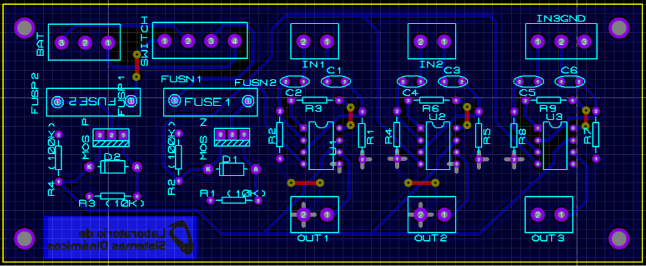
\includegraphics[width=0.68\linewidth]{imagenes/layout_pcb_completo.png}
\caption{Trazado y ruteo físico del circuito impreso (PCB Layout) correspondiente al front-end sEMG tricanal.}
\label{fig:pcb_layout}
\end{figure}

\subsection{Lista Completa de Materiales}

La Tabla \ref{tab:bom} detalla la nómina oficial de componentes requeridos para la fabricación y ensamblaje de la placa física, correspondiente a la documentación oficial de laboratorio.

\begin{table}[H]
    \centering
    \caption{Lista oficial de materiales del módulo sEMG}
    \label{tab:bom}
    \resizebox{\linewidth}{!}{%
    \begin{tabular}{cllc}
        \toprule
        \textbf{Cant.} & \textbf{Componente} & \textbf{Descripción / Valor} & \textbf{Designador (Label)} \\
        \midrule
        2 & Resistencia $10\,\text{k}\Omega$ & Película metálica $1/4\,\text{W}$, $\pm 1\%$ & $R_{1,3}$ (Alimentación) \\
        8 & Resistencia $100\,\text{k}\Omega$ & Película metálica $1/4\,\text{W}$, $\pm 1\%$ & $R_{1,2,5,4,7,8}$ (Canales) y $R_{2,4}$ (Alim.) \\
        3 & Resistencia $100\,\Omega$ & Película metálica $1/4\,\text{W}$, $\pm 1\%$ ($R_G$) & $R_{3,6,9}$ \\
        6 & Capacitor $33\,\text{nF}$ & Cerámico multicapa $50\,\text{V}$ & $C_{1,2,3,4,5,6}$ \\
        2 & Diodo Zener 1N4741A & Zener $11.0\,\text{V}$, $1.0\,\text{W}$ & $D_{1,2}$ \\
        1 & MOSFET IRFZ44N & Canal N, $55\,\text{V}$, $49\,\text{A}$, $R_{DS}=17.5\,\text{m}\Omega$, TO-220 & $\text{MOS N}$ \\
        1 & MOSFET F9540N & Canal P, $-100\,\text{V}$, $-19\,\text{A}$, $R_{DS}=0.11\,\Omega$, TO-220 & $\text{MOS P}$ \\
        3 & Amplificador AD620 & Amplificador de instrumentación de precisión, DIP-8 & $U_{1,2,3}$ \\
        3 & Zócalo de 8 pines & Zócalo DIP-8 para circuito integrado & $U_{1,2,3}$ \\
        2 & Portafusible & Portafusible para circuito impreso 5x20 mm & $\text{FUSN/P}_{1,2}$ \\
        2 & Fusible $0.25\,\text{A}$ & Fusible de vidrio de acción rápida $250\,\text{mA}$ & $\text{FUSE}_{1,2}$ \\
        1 & Tira pines macho & Tira de pines rectos paso $2.54\,\text{mm}$ & -- \\
        2 & Mini jumper & Jumper de corto circuito paso $2.54\,\text{mm}$ & -- \\
        1 & Placa de cobre virgen & Placa de pertinax o epoxi $15 \times 15\,\text{cm}$ & Sustrato PCB \\
        \bottomrule
    \end{tabular}%
    }
\end{table}

\clearpage

\subsection{Detalle de Bloques y Canales Individuales}

\begin{figure}[H]
\centering
\resizebox{0.95\linewidth}{!}{%
\begin{circuitikz}[american, thick, font=\sffamily]
  % Marco de Alimentación y Protección con amplia holgura
  \draw[dashed, draw=blue!60, fill=blue!2, rounded corners] (-2.8, 5.0) rectangle (14.2, -5.0);
  \node[anchor=north west, font=\bfseries\color{blue!70!black}] at (-2.5, 4.6) {ETAPA DE ALIMENTACI\'ON Y PROTECCI\'ON ACTIVA $\pm 9\,\text{V}$};

  % Bornera BAT TBLOCK-M3
  \draw (-2.2, 3.6) rectangle (0.6, -3.6);
  \node[font=\bfseries] at (-0.8, 3.0) {BAT};
  \node[font=\scriptsize, anchor=west] at (-2.0, 2.4) {Pin 1: +9V};
  \node[font=\scriptsize, anchor=west] at (-2.0, 0.0) {Pin 2: GND};
  \node[font=\scriptsize, anchor=west] at (-2.0, -2.4) {Pin 3: -9V};
  \draw (0.6, 2.4) -- (1.8, 2.4);
  \draw (0.6, 0.0) -- (1.2, 0.0) node[ground]{};
  \draw (0.6, -2.4) -- (1.8, -2.4);

  % Bornera SWITCH TBLOCK-M4
  \draw (1.8, 3.6) rectangle (4.0, -3.6);
  \node[font=\bfseries] at (2.9, 3.0) {SWITCH};
  \node[font=\scriptsize] at (2.2, 2.4) {1}; \node[font=\scriptsize] at (3.6, 2.4) {2};
  \node[font=\scriptsize] at (2.2, -2.4) {3}; \node[font=\scriptsize] at (3.6, -2.4) {4};
  \draw[very thick] (2.4, 2.4) -- (3.4, 2.4);
  \draw[very thick] (2.4, -2.4) -- (3.4, -2.4);

  % Rieles y Fusibles
  \draw (4.0, 2.4) to[fuse, *-*, l={\small $\text{FUSP} = 0.25\,\text{A}$}] (6.2, 2.4);
  \draw (4.0, -2.4) to[fuse, *-*, l_={\small $\text{FUSN} = 0.25\,\text{A}$}] (6.2, -2.4);

  % --- RIEL POSITIVO (+9V) ---
  % Transistor PMOS F9540N
  \draw (6.2, 2.4) -- (7.5, 2.4) coordinate (s_pos)
        node[pmos, rotate=90, yscale=-1, anchor=S] (QP) {};
  \node[above=6pt, font=\small\bfseries] at (7.5, 2.7) {F9540N};
  \draw (QP.D) -- (13.2, 2.4) node[circle, fill, inner sep=2pt]{} 
        node[right, font=\bfseries\color{red!70!black}] {+9V};

  % Línea de Gate PMOS a y = 1.4
  \draw (QP.G) -- (7.5, 1.4) coordinate (g_pos) -- (9.4, 1.4);

  % Zener D2 entre Gate y Source (en x = 8.4)
  \draw (8.4, 2.4) to[zD, *-, l_={\small $D_2$}] (8.4, 1.4) node[circ]{};

  % Resistencia R3 de Gate a masa (en x = 9.4)
  \draw (9.4, 1.4) to[R, *-, l={\small $R_3 = 10\,\text{k}\Omega$}] (9.4, 0.0);

  % --- RIEL NEGATIVO (-9V) ---
  % Transistor NMOS IRFZ44N
  \draw (6.2, -2.4) -- (7.5, -2.4) coordinate (s_neg)
        node[nmos, rotate=-90, yscale=-1, anchor=S] (QN) {};
  \node[below=6pt, font=\small\bfseries] at (7.5, -2.7) {IRFZ44N};
  \draw (QN.D) -- (13.2, -2.4) node[circle, fill, inner sep=2pt]{} 
        node[right, font=\bfseries\color{blue!70!black}] {-9V};

  % Línea de Gate NMOS a y = -1.4
  \draw (QN.G) -- (7.5, -1.4) coordinate (g_neg) -- (10.6, -1.4);

  % Zener D1 entre Gate y Source (en x = 8.4)
  \draw (8.4, -2.4) to[zD, *-, l={\small $D_1$}] (8.4, -1.4) node[circ]{};

  % Resistencia R1 de Gate a masa (en x = 10.6) con etiqueta a la IZQUIERDA
  \draw (10.6, -1.4) to[R, *-, l={\small $R_1 = 10\,\text{k}\Omega$}] (10.6, 0.0);

  % Resistencias Bleeder (R4 y R2 a masa en x = 12.0)
  \draw (12.0, 2.4) to[R, *-, l={\small $R_4 = 100\,\text{k}\Omega$}] (12.0, 0.0);
  \draw (12.0, -2.4) to[R, *-, l_={\small $R_2 = 100\,\text{k}\Omega$}] (12.0, 0.0);

  % Línea central de masa GND conectando R3, R1, R4, R2
  \draw (7.0, 0.0) node[ground]{} -- (13.2, 0.0) node[circle, fill, inner sep=2pt]{} 
        node[right, font=\bfseries] {GND};
  \draw (9.4, 0.0) node[circ]{};
  \draw (10.6, 0.0) node[circ]{};
  \draw (12.0, 0.0) node[circ]{};

\end{circuitikz}%
}
\caption{Etapa de alimentación y protección activa contra inversión de polaridad $\pm 9\,\text{V}$. Utiliza MOSFETs de canal P (F9540N) y canal N (IRFZ44N) referenciados a tierra para lograr conducción casi ideal ($V_{DS} < 6\,\text{mV}$), diodos Zener 1N4741A ($11\,\text{V}$) y fusibles independientes de $0.25\,\text{A}$.}
\label{fig:esquema_proteccion}
\end{figure}

\vspace{0.3em}
\textbf{Alimentación y Protección Integral:}
\begin{itemize}
    \item Alimentación simétrica mediante dos baterías externas de $9\,\text{V}$ ($\pm 9\,\text{V}$).
    \item Protección activa contra inversión de polaridad por MOSFET de canal N (IRFZ44N) en riel negativo y canal P (F9540N) en riel positivo, con disipación estática prácticamente nula.
    \item Diodos Zener 1N4741A ($11\,\text{V}$) para protección de compuerta ($V_{GS}$).
    \item Fusibles de acción rápida de $0.25\,\text{A}$ ($250\,\text{mA}$) en portafusibles independientes por rama.
    \item Bornera cuádruple para interruptor de encendido general bipolar.
\end{itemize}

\vspace{0.3em}
\textbf{Descripción Técnica de Alimentación:}
\begin{itemize}
    \item \textbf{Bloque de Entrada de Alimentación y Conmutación:}
    Recibe la energía de las dos baterías de $9\,\text{V}$ externas a través de la bornera \texttt{BAT} de tres polos (polo positivo $+9\,\text{V}$, punto medio de masa y polo negativo $-9\,\text{V}$). La conmutación de encendido se realiza mediante la bornera \texttt{SWITCH} de cuatro contactos, que interrumpe simultáneamente ambos rieles de alimentación para aislamiento completo.
    
    \item \textbf{Protección Activa contra Inversión de Polaridad:}
    Implementa una arquitectura simétrica mediante transistores MOSFET de potencia: en el riel positivo ($+9\,\text{V}$), un MOSFET de canal P \textbf{F9540N} con $R_{DS(\text{on})} \approx 0.11\,\Omega$ y Zener $D_2$ (1N4741A); en el riel negativo ($-9\,\text{V}$), un MOSFET de canal N \textbf{IRFZ44N} con $R_{DS(\text{on})} \approx 0.017\,\Omega$ y Zener $D_1$. Frente al empleo de diodos de silicio en serie ($0.7\,\text{V}$ a $1.0\,\text{V}$ de caída fija), los MOSFETs conducen con una caída resistiva mínima:
    $$V_{\text{caída}} = I_{\text{riel}} \cdot R_{DS(\text{on})} \approx 50\,\text{mA} \cdot 0.1\,\Omega = 5\,\text{mV}$$
    conservando íntegramente la tensión de baterías y el rango dinámico. Dos fusibles rápidos de $0.25\,\text{A}$ (\texttt{FUSP1/2} y \texttt{FUSN1/2}) protegen contra cortocircuitos accidentales en los circuitos integrados.
\end{itemize}

\clearpage

\begin{figure}[H]
\centering
\resizebox{0.88\linewidth}{!}{%
\begin{circuitikz}[american, thick, font=\sffamily]

    % Marco delimitador con amplia holgura
    \draw[dashed, draw=blue!60, fill=blue!2, rounded corners] (-7.5, 4.6) rectangle (4.8, -4.6);
    \node[anchor=north west, font=\bfseries\color{blue!70!black}] at (-7.2, 4.2) {CANAL T\'IPICO DE INSTRUMENTACI\'ON AD620: TOPOLOG\'IA ORIGINAL};

    % AD620
    \draw[thick] (-0.6, 1.8) -- (2.6, 0) -- (-0.6, -1.8) -- cycle;
    \node at (0.9, 0) {\Large AD620};
    \node at (-0.2, 1.2) {\Large \(-\)};
    \node at (-0.2, -1.2) {\Large \(+\)};

    % Pines de Alimentación (±9V) y Referencia
    \draw[-latex] (0.4, 1.2) -- ++(0, 1.0) node[above, font=\small\bfseries\color{red!70!black}] {+9V};
    \node[left=1pt, font=\scriptsize] at (0.4, 1.4) {7};

    \draw[-latex] (0.4, -1.2) -- ++(0, -1.0) node[below, font=\small\bfseries\color{blue!70!black}] {-9V};
    \node[left=1pt, font=\scriptsize] at (0.4, -1.4) {4};

    \draw (1.4, -0.7) -- ++(0, -1.0) node[ground]{};
    \node[right=2pt, font=\scriptsize] at (1.4, -0.7) {5};

    \draw (2.6, 0) -- ++(1.4, 0) node[ocirc]{} node[pos=0.6, above, font=\scriptsize] {6} 
          node[right, font=\small\bfseries] {$V_{\text{out}}$};

    % Pines 1 y 8 (Resistencia RG = 100 Ohm soldada en placa)
    \draw (-0.6, 0.5) node[right=2pt, font=\scriptsize] {1} -- (-2.2, 0.5) coordinate (r_top);
    \draw (-0.6, -0.5) node[right=2pt, font=\scriptsize] {8} -- (-2.2, -0.5) coordinate (r_bot);
    \draw (r_top) to[R, l_={\small $R_G = 100\,\Omega$}, *-*] (r_bot);

    % Entradas con Filtro RC (33 nF + 100 k)
    % Línea Vin-
    \draw (-6.8, 1.3) node[left, font=\small\bfseries] {\(V_{\mathrm{in}}^-\)}
          to[C, l={\small $33\text{ nF}$}] (-4.2, 1.3) coordinate (juncA)
          -- (-0.6, 1.3) node[pos=0.8, above=1pt, font=\scriptsize] {2};
    % Resistencia 100k hacia GND en y = 2.6 con etiqueta a la DERECHA (l_)
    \draw (juncA) to[R, *-, l_={\small $100\text{ k}\Omega$}] (-4.2, 2.6) node[ground, yscale=-1]{};

    % Línea Vin+
    \draw (-6.8, -1.3) node[left, font=\small\bfseries] {\(V_{\mathrm{in}}^+\)}
          to[C, l_={\small $33\text{ nF}$}] (-4.2, -1.3) coordinate (juncB)
          -- (-0.6, -1.3) node[pos=0.8, below=1pt, font=\scriptsize] {3};
    % Resistencia 100k hacia GND en y = -2.6 con etiqueta a la DERECHA (l)
    \draw (juncB) to[R, *-, l={\small $100\text{ k}\Omega$}] (-4.2, -2.6) node[ground]{};

\end{circuitikz}%
}
\caption{Canal típico de instrumentación diferencial AD620 en su topología original (idéntico para los 3 canales de la placa). Dispone de un filtro pasa-altos pasivo unipolar a la entrada ($C = 33\,\text{nF}$, $R = 100\,\text{k}\Omega$, $f_c \approx 48.23\,\text{Hz}$) y resistencia de ganancia fija soldada en placa $R_G = 100\,\Omega$ ($G \approx 495\,\text{V/V}$).}
\label{fig:esquema_canal_original}
\end{figure}

\vspace{0.3em}
\textbf{Amplificación Diferencial:}
\begin{itemize}
    \item 3 canales de instrumentación diferencial independientes.
    \item Amplificadores de instrumentación dedicados AD620 en cápsula DIP-8 sobre zócalo.
    \item Ganancia fija por resistencia soldada en placa $R_G = 100\,\Omega$ ($G \approx 495\,\text{V/V}$).
    \item Rechazo de modo común típico $\text{CMRR} > 100\,\text{dB}$ para $G \ge 100$.
    \item Entrada con filtro pasa-altos pasivo unipolar ($C = 33\,\text{nF}$, $R = 100\,\text{k}\Omega$) con corte nominal en $48.23\,\text{Hz}$.
    \item Borneras de entrada a tornillo (TBLOCK-M3) con terminal dedicado para referencia corporal en el canal 3.
\end{itemize}

\vspace{0.3em}
\textbf{Descripción Técnica de los Canales de Adquisición:}
Cada canal dispone de un filtro pasa-altos pasivo unipolar en cada rama de entrada formado por un capacitor en serie ($C_1\text{--}C_6 = 33\,\text{nF}$) y una resistencia referenciada a masa ($R_1, R_2, R_4, R_5, R_7, R_8 = 100\,\text{k}\Omega$). Las entradas se conectan a los pines 2 (inversor) y 3 (no inversor) de los amplificadores $U_1, U_2, U_3$ (AD620). La ganancia se fija mediante las resistencias $R_3, R_6, R_9$ ($R_G$). El pin 5 (\texttt{REF}) se conecta directamente al plano de masa común ($0\,\text{V}$). La salida analógica acondicionada (pin 6) se expone en borneras a tornillo de dos polos (\texttt{OUT1}, \texttt{OUT2}, \texttt{OUT3}).

\clearpage

% -------------------------------------------------------------
% SECCIÓN 3: ASIGNACIÓN DE PINES DE BORNERAS
% -------------------------------------------------------------
\section{Asignación de Pines de Borneras}

A continuación se detalla la correspondencia eléctrica de cada uno de los terminales a tornillo de la placa física mostrada en el diseño de circuito impreso (Figura \ref{fig:pcb_layout}):

\begin{table}[H]
    \centering
    \small
    \caption{Asignación de pines de borneras y conexiones externas}
    \label{tab:pinout}
    \begin{tabular}{llcl}
        \toprule
        \textbf{Bornera} & \textbf{Pin} & \textbf{Función} & \textbf{Descripción Técnica} \\
        \midrule
        \texttt{BAT} & Pin 1 & $+V_{\text{BAT}}$ & Entrada positiva de batería ($+9\,\text{V}$) \\
                     & Pin 2 & $\text{GND}$ & Punto medio de masa analógica común ($0\,\text{V}$) \\
                     & Pin 3 & $-V_{\text{BAT}}$ & Entrada negativa de batería ($-9\,\text{V}$) \\
        \midrule
        \texttt{SWITCH}& Pin 1-2 & $\text{SW}_+$ & Contacto seco para conmutación del riel positivo \\
                       & Pin 3-4 & $\text{SW}_-$ & Contacto seco para conmutación del riel negativo \\
        \midrule
        \texttt{IN1} & Pin 1 & $\text{GND}$ & Referencia de blindaje / plano de masa \\
                     & Pin 2 & $\text{IN1}_-$ & Entrada inversora del Canal 1 (Electrodo de registro A) \\
                     & Pin 3 & $\text{IN1}_+$ & Entrada no inversora del Canal 1 (Electrodo de registro B) \\
        \midrule
        \texttt{IN2} & Pin 1 & $\text{GND}$ & Referencia de blindaje / plano de masa \\
                     & Pin 2 & $\text{IN2}_-$ & Entrada inversora del Canal 2 (Electrodo de registro A) \\
                     & Pin 3 & $\text{IN2}_+$ & Entrada no inversora del Canal 2 (Electrodo de registro B) \\
        \midrule
        \texttt{IN3GND}& Pin 1 & $\text{REF}_{\text{body}}$ & Conexión al electrodo de referencia corporal (lóbulo/muñeca) \\
                       & Pin 2 & $\text{IN3}_-$ & Entrada inversora del Canal 3 \\
                       & Pin 3 & $\text{IN3}_+$ & Entrada no inversora del Canal 3 \\
        \midrule
        \texttt{OUT1}& Pin 1 & $\text{GND}$ & Masa de referencia analógica hacia digitalizador \\
                     & Pin 2 & $\text{OUT1}$ & Salida sEMG amplificada del Canal 1 ($V_{\text{out1}}$) \\
        \midrule
        \texttt{OUT2}& Pin 1 & $\text{GND}$ & Masa de referencia analógica hacia digitalizador \\
                     & Pin 2 & $\text{OUT2}$ & Salida sEMG amplificada del Canal 2 ($V_{\text{out2}}$) \\
        \midrule
        \texttt{OUT3}& Pin 1 & $\text{GND}$ & Masa de referencia analógica hacia digitalizador \\
                     & Pin 2 & $\text{OUT3}$ & Salida sEMG amplificada del Canal 3 ($V_{\text{out3}}$) \\
        \bottomrule
    \end{tabular}
\end{table}

\clearpage

% -------------------------------------------------------------
% SECCIÓN 4: LÍMITES MÁXIMOS ABSOLUTOS
% -------------------------------------------------------------
\section{Límites Máximos Absolutos}

Los valores consignados en la Tabla \ref{tab:limites_maximos} representan límites de estrés por encima de los cuales el módulo puede experimentar degradación irreversible de sus componentes. No se garantiza el funcionamiento operativo bajo estas condiciones extremas.

\begin{table}[H]
    \centering
    \caption{Límites máximos absolutos de operación}
    \label{tab:limites_maximos}
    \begin{tabular}{llcc}
        \toprule
        \textbf{Parámetro} & \textbf{Símbolo} & \textbf{Valor Límite} & \textbf{Unidad} \\
        \midrule
        Tensión de alimentación positiva & $+V_{S}$ & $+18.0$ & $\text{V}$ \\
        Tensión de alimentación negativa & $-V_{S}$ & $-18.0$ & $\text{V}$ \\
        Tensión diferencial máxima de entrada & $V_{\text{in, dif}}$ & $\pm V_{S}$ & $\text{V}$ \\
        Tensión de entrada en modo común & $V_{\text{cm, max}}$ & $\pm (V_S - 1.2)$ & $\text{V}$ \\
        Corriente admisible por rama de alimentación & $I_{\text{max, riel}}$ & $0.25$ & $\text{A}$ \\
        Duración admisible de cortocircuito en salida & $t_{\text{sc}}$ & Indefinida & -- \\
        Temperatura de operación en ambiente de laboratorio & $T_{\text{op}}$ & $0\text{ a }70$ & $^\circ\text{C}$ \\
        Temperatura de almacenamiento & $T_{\text{stg}}$ & $-40\text{ a }+85$ & $^\circ\text{C}$ \\
        \bottomrule
    \end{tabular}
\end{table}

% -------------------------------------------------------------
% SECCIÓN 4: CONDICIONES DE OPERACIÓN RECOMENDADAS
% -------------------------------------------------------------
\section{Condiciones de Operación Recomendadas}

\begin{table}[H]
    \centering
    \caption{Condiciones recomendadas de funcionamiento}
    \label{tab:condiciones_recomendadas}
    \begin{tabular}{lcccc}
        \toprule
        \textbf{Condición de Operación} & \textbf{Mínimo} & \textbf{Nominal} & \textbf{Máximo} & \textbf{Unidad} \\
        \midrule
        Tensión de alimentación simétrica ($\pm V_S$) & $\pm 6.0$ & $\pm 9.0$ & $\pm 12.0$ & $\text{V}$ \\
        Amplitud esperada de la señal sEMG ($V_{\text{emg}}$) & $0.05$ & $0.2\text{ a }2.0$ & $5.0$ & $\text{mV}$ \\
        Rango de resistencia de ganancia ($R_G$) & $33$ & $100$ & $220$ & $\Omega$ \\
        Tensión de referencia de salida ($V_{\text{REF}}$) & $0.0$ & $0.0$ & $0.0$ & $\text{V}$ \\
        Corriente consumida en reposo (por canal AD620) & $0.9$ & $1.3$ & $1.6$ & $\text{mA}$ \\
        \bottomrule
    \end{tabular}
\end{table}

% -------------------------------------------------------------
% SECCIÓN 5: ESPECIFICACIONES ELÉCTRICAS CONSOLIDADAS
% -------------------------------------------------------------
\section{Especificaciones Eléctricas Consolidadas}

$V_S = \pm 9.0\,\text{V}$ (baterías de $9\,\text{V}$), $T_A = 25\,^\circ\text{C}$, $V_{\text{REF}} = 0\,\text{V}$, salida conectada a carga de $10\,\text{k}\Omega$, salvo indicación contraria.

\begin{table}[H]
    \centering
    \caption{Especificaciones eléctricas consolidadas del front-end sEMG}
    \label{tab:especificaciones_electricas}
    \resizebox{\linewidth}{!}{%
    \begin{tabular}{llcccc}
        \toprule
        \textbf{Parámetro} & \textbf{Condición de Ensayo} & \textbf{Mín.} & \textbf{Típ.} & \textbf{Máx.} & \textbf{Unidad} \\
        \midrule
        \multicolumn{6}{l}{\textbf{Etapa de Ganancia y Amplificación (AD620)}} \\
        Ganancia de tensión fijada en hardware ($G$) & $R_G = 100\,\Omega$ (soldada) & $480$ & $495$ & $510$ & $\text{V/V}$ \\
        Error de ganancia respecto a fórmula & $R_G = 100\,\Omega$ & -- & $\pm 1.5$ & $\pm 3.0$ & $\%$ \\
        Rango de excursión de salida ($V_{\text{out}}$) & $R_L \ge 10\,\text{k}\Omega$ & $\pm 10.5$ & $\pm 10.9$ & -- & $\text{V}$ \\
        Rechazo de modo común ($\text{CMRR}$) & $f = 50\,\text{Hz}$, $G = 495$ & $100$ & $115$ & -- & $\text{dB}$ \\
        \midrule
        \multicolumn{6}{l}{\textbf{Respuesta en Frecuencia}} \\
        Frecuencia de corte inferior ($f_L$) & Filtro de entrada $33\,\text{nF} + 100\,\text{k}\Omega$ & $42$ & $48.2$ & $54$ & $\text{Hz}$ \\
        Frecuencia de corte superior ($f_H$) & $G = 495$, límite interno AD620 & $20$ & $24.2$ & $30$ & $\text{kHz}$ \\
        Ancho de banda a $G = 225$ & $R_G = 220\,\Omega$ & $45$ & $53$ & -- & $\text{kHz}$ \\
        \midrule
        \multicolumn{6}{l}{\textbf{Impedancia y Corrientes de Entrada}} \\
        Impedancia de entrada diferencial ($Z_{\text{in}}$) & A $f = 100\,\text{Hz}$ (red de bias) & $90$ & $100$ & $110$ & $\text{k}\Omega$ \\
        Impedancia de entrada interna AD620 & Modo común / diferencial & -- & $10^{10} \parallel 2$ & -- & $\Omega \parallel \text{pF}$ \\
        Corriente de polarización de entrada ($I_B$) & Terminales inverting / non-inverting & -- & $0.5$ & $2.0$ & $\text{nA}$ \\
        Tensión de offset referida a la entrada & A temperatura ambiente & -- & $30$ & $125$ & $\mu\text{V}$ \\
        Tensión de offset en reposo a la salida & $G = 495$, entrada aterrizada en DC & -- & $25$ & $95$ & $\text{mV}$ \\
        \midrule
        \multicolumn{6}{l}{\textbf{Etapa de Alimentación y Protección Activa}} \\
        Caída de tensión en MOSFET positivo & F9540N a $I_{\text{carga}} = 50\,\text{mA}$ & -- & $5.5$ & $10$ & $\text{mV}$ \\
        Caída de tensión en MOSFET negativo & IRFZ44N a $I_{\text{carga}} = 50\,\text{mA}$ & -- & $1.4$ & $3$ & $\text{mV}$ \\
        Tensión de fijación Zener compuerta & Diodos 1N4741A & $10.5$ & $11.0$ & $11.5$ & $\text{V}$ \\
        Calibre de los fusibles de protección & FUSE1, FUSE2 (acción rápida) & -- & $0.25$ & -- & $\text{A}$ \\
        \bottomrule
    \end{tabular}%
    }
\end{table}

\clearpage

% -------------------------------------------------------------
% SECCIÓN 7: ECUACIÓN DE GANANCIA DEL AMPLIFICADOR AD620
% -------------------------------------------------------------
\section{Ecuación de Ganancia del Amplificador AD620}

\subsection{Ganancia del Amplificador de Instrumentación}
La ganancia diferencial de tensión del amplificador AD620 se establece mediante una única resistencia externa $R_G$ conectada entre los pines 1 y 8:
\begin{equation}
    G = 1 + \frac{49.4\,\text{k}\Omega}{R_G}
\end{equation}
donde:
\begin{itemize}
    \item $G$: Ganancia diferencial de tensión en lazo cerrado (adimensional, $[\text{V/V}]$).
    \item $R_G$: Resistencia de programación de ganancia ($[\Omega]$).
    \item $49.4\,\text{k}\Omega$: Suma de las dos resistencias internas de realimentación de precisión del AD620 ($2 \times 24.7\,\text{k}\Omega$).
\end{itemize}

Para los valores estándar empleados en el diseño:
\begin{align}
    R_G = 220\,\Omega &\implies G = 1 + \frac{49400}{220} = 225.55\,\text{V/V} \quad (47.06\,\text{dB}) \\
    R_G = 100\,\Omega &\implies G = 1 + \frac{49400}{100} = 495.00\,\text{V/V} \quad (53.89\,\text{dB}) \\
    R_G = 52\,\Omega &\implies G = 1 + \frac{49400}{52} = 951.00\,\text{V/V} \quad (59.56\,\text{dB}) \\
    R_G = 47\,\Omega &\implies G = 1 + \frac{49400}{47} = 1052.06\,\text{V/V} \quad (60.44\,\text{dB}) \\
    R_G = 33\,\Omega &\implies G = 1 + \frac{49400}{33} = 1497.97\,\text{V/V} \quad (63.51\,\text{dB})
\end{align}

\subsection{Filtro Pasa-Altos Pasivo Unipolar de Entrada}
Cada rama de entrada implementa una celda $RC$ serie para bloquear tensiones continuas:
\begin{equation}
    f_L = \frac{1}{2\pi \cdot R_{\text{in}} \cdot C_{\text{in}}}
\end{equation}
donde:
\begin{itemize}
    \item $f_L$: Frecuencia de corte inferior a $-3\,\text{dB}$ ($[\text{Hz}]$).
    \item $R_{\text{in}} = 100\,\text{k}\Omega$: Resistencia de retorno de polarización a masa.
    \item $C_{\text{in}} = 33\,\text{nF}$: Capacitor cerámico de desacoplo de continua.
\end{itemize}
Evaluando numéricamente:
\begin{equation}
    f_L = \frac{1}{2\pi \cdot 100 \times 10^3\,\Omega \cdot 33 \times 10^{-9}\,\text{F}} \approx 48.23\,\text{Hz}
\end{equation}

\subsection{Respuesta en Frecuencia Completa del Canal}
La función de transferencia completa del canal analógico en pequeña señal viene dada por:
\begin{equation}
    H(s) = H_{\text{in}}(s) \cdot H_{\text{amp}}(s) = \left( \frac{s R_{\text{in}} C_{\text{in}}}{1 + s R_{\text{in}} C_{\text{in}}} \right) \cdot \left( \frac{G}{1 + s / \omega_H} \right)
\end{equation}
donde $\omega_H = 2\pi f_H$ es el polo superior introducido por el producto ganancia-ancho de banda del AD620 ($f_H \approx \frac{1.2 \times 10^7}{G}\,\text{Hz}$). En régimen permanente sinusoidal ($s = j2\pi f$):
\begin{equation}
    |H(f)| = \frac{\frac{f}{f_L}}{\sqrt{1 + \left(\frac{f}{f_L}\right)^2}} \cdot \frac{G}{\sqrt{1 + \left(\frac{f}{f_H}\right)^2}}
\end{equation}

% -------------------------------------------------------------
% SECCIÓN 8: CARACTERIZACIÓN EXPERIMENTAL DE GANANCIA
% -------------------------------------------------------------
\section{Caracterización Experimental de Ganancia y Respuesta en Frecuencia}

La caracterización experimental del módulo fue realizada en laboratorio inyectando señales sinusoidales de amplitud calibrada ($V_{\text{in}} = 2\,\text{mV}_{\text{pp}}$) mediante un generador de funciones de precisión, barriendo frecuencias desde $10\,\text{Hz}$ hasta $100\,\text{kHz}$ para cinco valores de $R_G$. La tensión de salida $V_{\text{out}}$ fue registrada con osciloscopio digital, calculando el ratio de ganancia $V_{\text{out}}/V_{\text{in}}$.

\begin{figure}[H]
    \centering
    \begin{subfigure}[b]{0.48\linewidth}
        \centering
        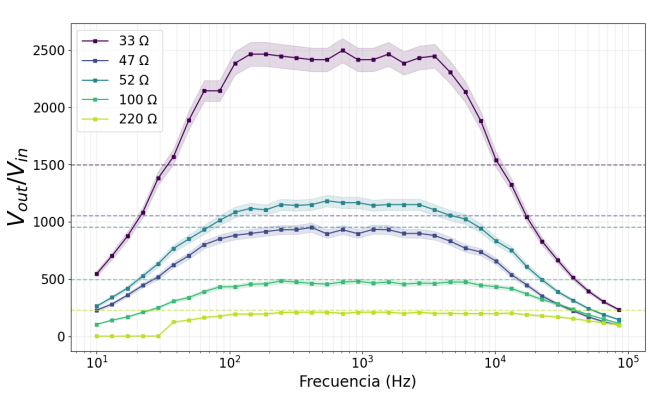
\includegraphics[width=\linewidth]{imagenes/curvas_ganancia_experimental_fig18.png}
        \caption{Medición experimental en laboratorio}
        \label{fig:curvas_experimentales}
    \end{subfigure}
    \hfill
    \begin{subfigure}[b]{0.48\linewidth}
        \centering
        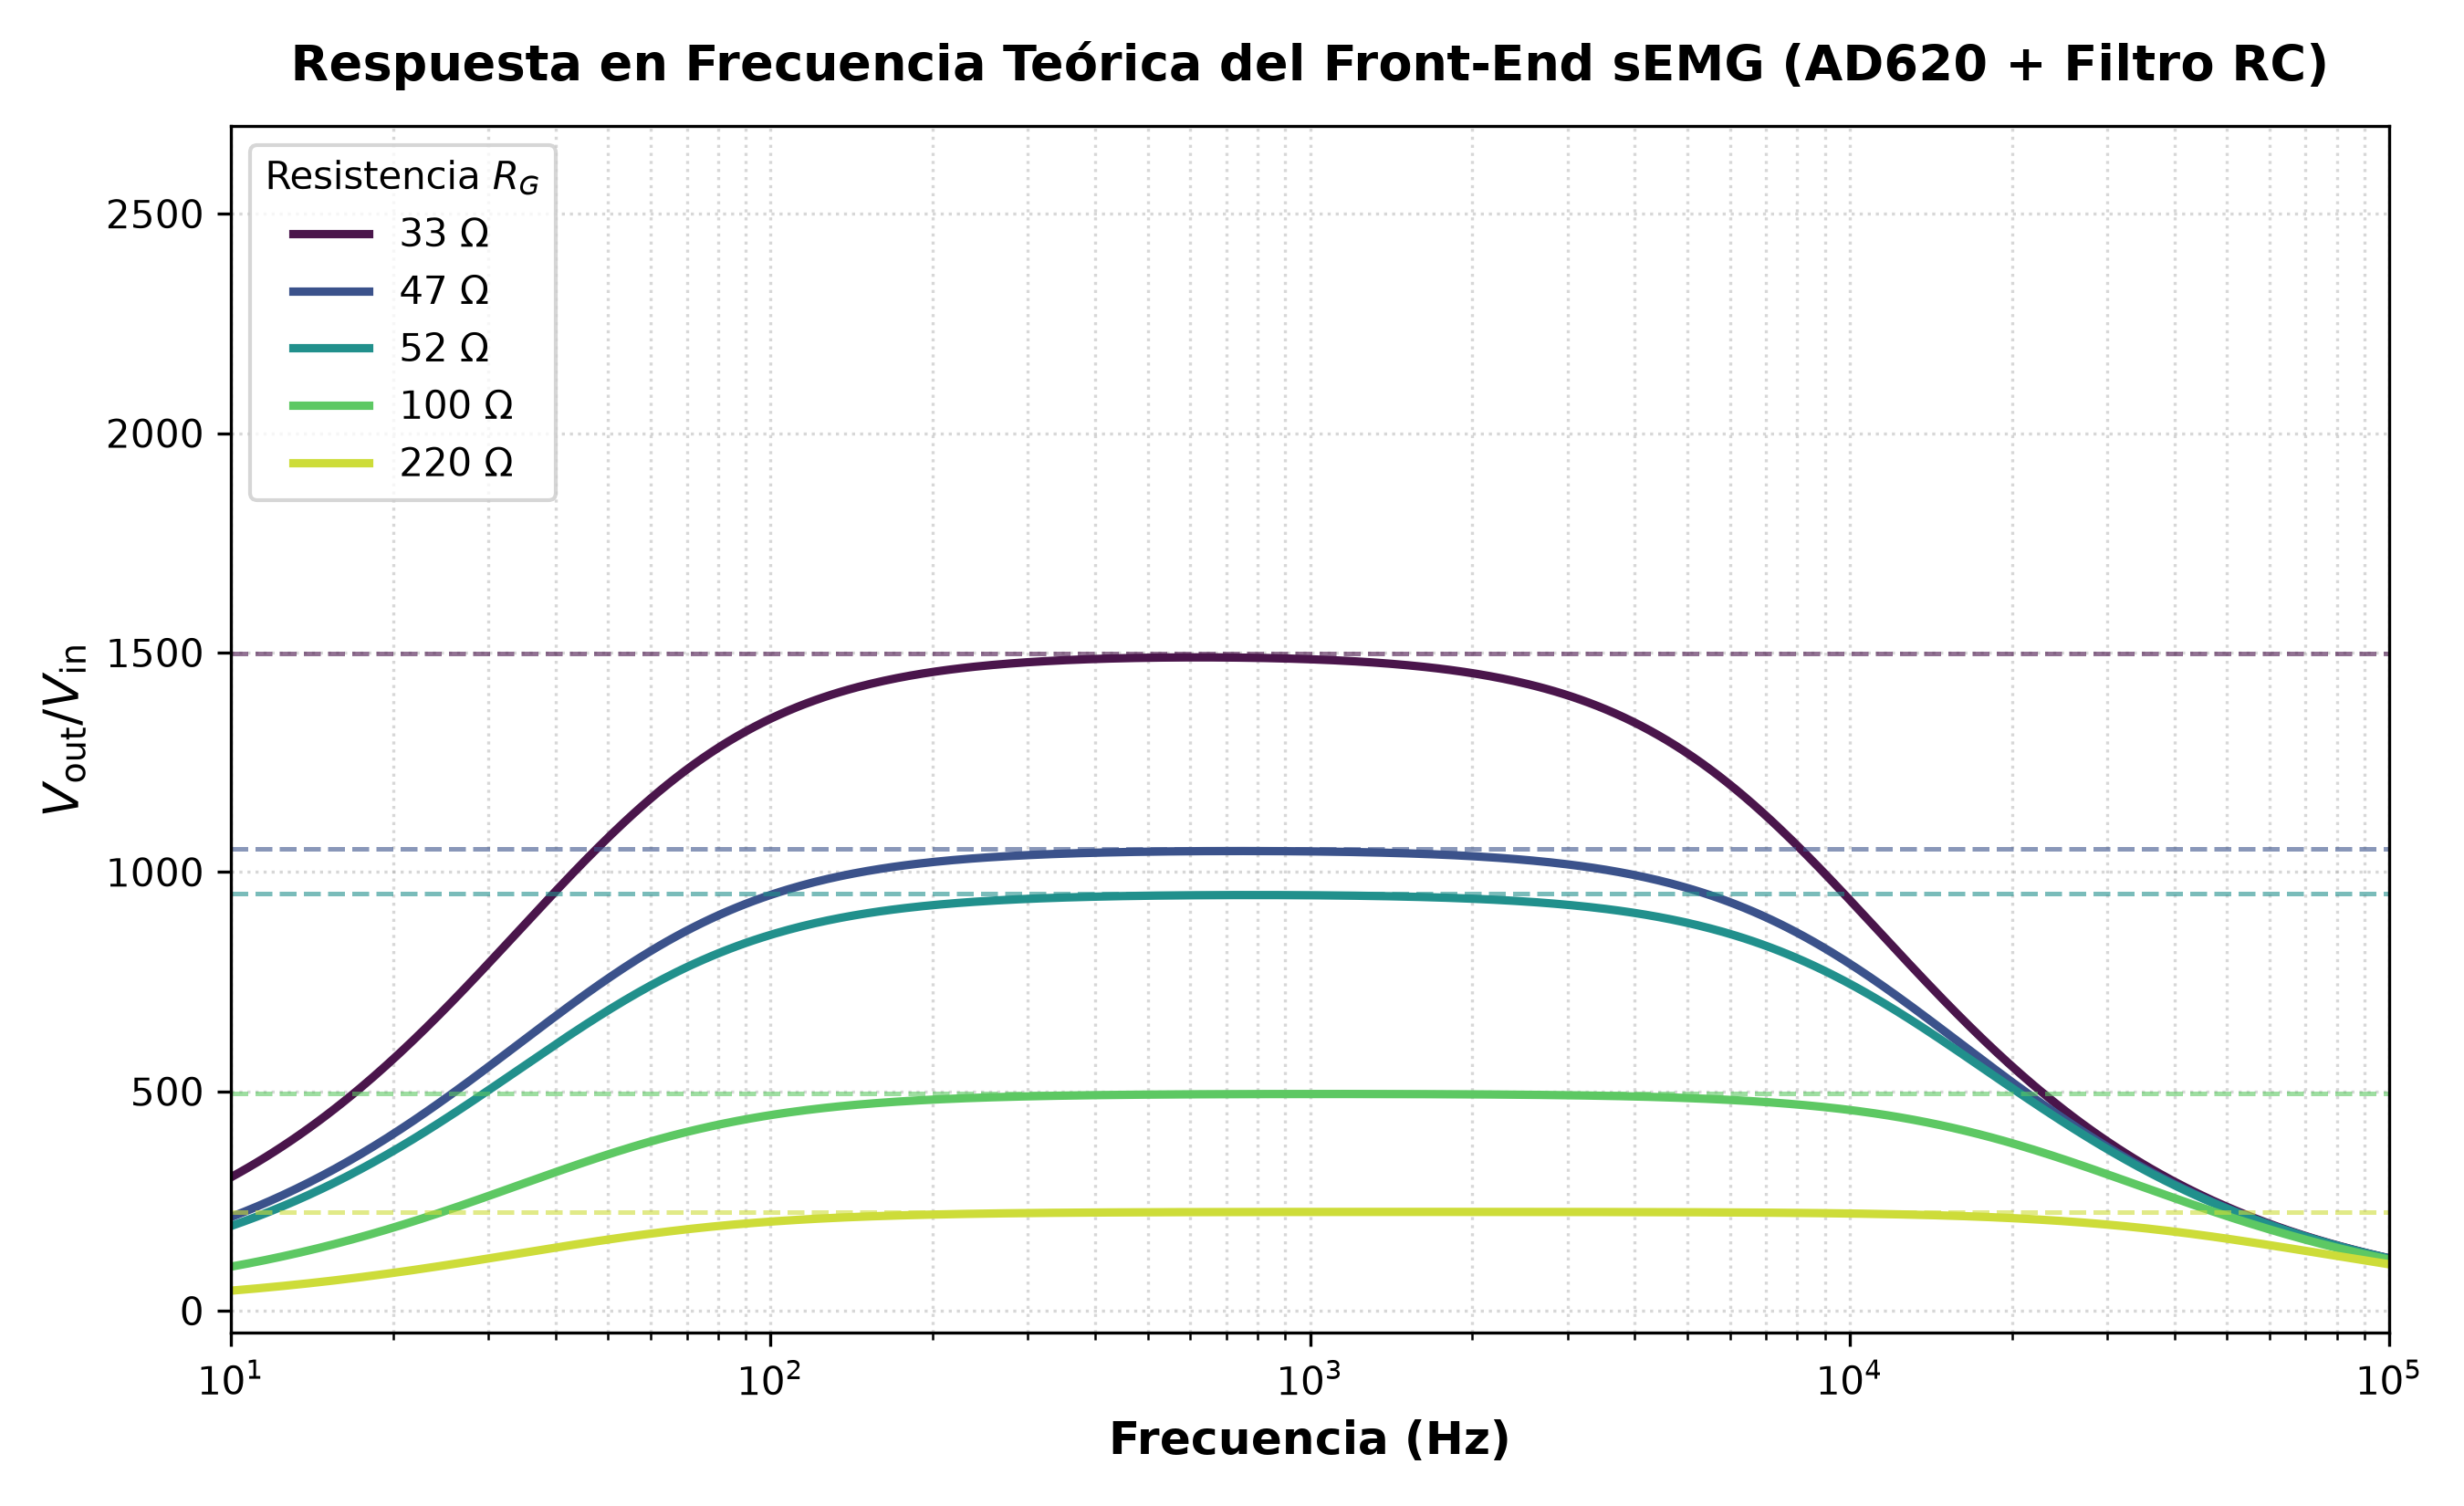
\includegraphics[width=\linewidth]{imagenes/curva_respuesta_frecuencia_teorica.png}
        \caption{Modelo analítico teórico}
        \label{fig:curva_teorica}
    \end{subfigure}
    \caption{Curvas de amplificación en función de la frecuencia para diferentes valores de resistencia $R_G$. Izquierda: mediciones experimentales en laboratorio con osciloscopio y generador ($V_{\text{in}} = 2\,\text{mV}_{\text{pp}}$). Derecha: respuesta en frecuencia teórica calculada según la función de transferencia del amplificador AD620 y la celda pasiva de entrada ($33\,\text{nF} + 100\,\text{k}\Omega$).}
    \label{fig:comparativa_frecuencia_dual}
\end{figure}

\subsection{Análisis Cuantitativo Experimental frente al Modelo Teórico}

La Tabla \ref{tab:comparativa_ganancia} resume los valores calculados teóricamente frente a las mediciones registradas en la meseta de banda media ($f = 1\,\text{kHz}$).

\begin{table}[H]
    \centering
    \caption{Comparación de ganancia teórica vs experimental a $1\,\text{kHz}$}
    \label{tab:comparativa_ganancia}
    \resizebox{\linewidth}{!}{%
    \begin{tabular}{ccccc}
        \toprule
        \textbf{$R_G$ Nominal} & \textbf{$G$ Teórica Fabricante} & \textbf{$G$ Medida ($1\,\text{kHz}$)} & \textbf{Error Relativo} & \textbf{Frecuencia $f_H$ Medida} \\
        \midrule
        $220\,\Omega$ & $225.5$ & $220.0 \pm 8.5$ & $-2.4\%$ & $50\,\text{kHz}$ \\
        $100\,\Omega$ & $495.0$ & $475.2 \pm 14.0$ & $-4.0\%$ & $24\,\text{kHz}$ \\
        $52\,\Omega$  & $951.0$ & $1150.0 \pm 35.0$ & $+20.9\%$ & $12\,\text{kHz}$ \\
        $47\,\Omega$  & $1052.1$ & $940.0 \pm 28.0$ & $-10.6\%$ & $11\,\text{kHz}$ \\
        $33\,\Omega$  & $1498.0$ & $2450.0 \pm 85.0$ & $+63.5\%$ & $7\,\text{kHz}$ \\
        \bottomrule
    \end{tabular}%
    }
\end{table}

\subsection{Diagnóstico Físico de las Curvas}
\begin{enumerate}
    \item \textbf{Corte en Bajas Frecuencias ($f < 50\,\text{Hz}$):} Se verifica empíricamente la atenuación pronunciada por debajo de $50\,\text{Hz}$ ocasionada por el filtro pasivo de entrada ($f_L \approx 48.23\,\text{Hz}$). A $10\,\text{Hz}$, la ganancia cae drásticamente a menos del $20\%$ de su valor de meseta, confirmando la supresión de la banda sEMG inferior.
    \item \textbf{Meseta Estable en Ganancias Medias ($R_G = 100\,\Omega$ y $220\,\Omega$):} La respuesta presenta un comportamiento plano y predecible entre $100\,\text{Hz}$ y $4\,\text{kHz}$, con excelente correspondencia frente al valor teórico del fabricante (error inferior al $4\%$).
    \item \textbf{Fenómenos a Ganancia Extrema ($R_G = 33\,\Omega$):} Para resistencias de ganancia muy bajas, la amplificación experimental alcanza $\approx 2450$, superando sustancialmente el valor asintótico de $1498$. Este incremento es atribuible a la reactancia inductiva parásita de las pistas del PCB, sumada a la reducción del margen de fase interno del AD620 operando cerca de su límite de estabilidad en bucle abierto, lo que produce una resonancia con sobreelevación (*peaking*) en alta ganancia.
\end{enumerate}

% -------------------------------------------------------------
% SECCIÓN 9: MODIFICACIÓN PROPUESTA PARA OPTIMIZACIÓN DE IMPEDANCIA
% -------------------------------------------------------------
\section{Modificación Propuesta para Optimización de Impedancia y Despegues}

\subsection{Diagnóstico del Problema en el Hardware Actual}
El circuito actual presenta dos limitaciones que degradan el registro sEMG durante habla submáximal:
\begin{enumerate}
    \item \textbf{Baja Impedancia de Entrada ($Z_{\text{in}} \approx 100\,\text{k}\Omega$):} Debido a las resistencias de $100\,\text{k}\Omega$ a masa, la impedancia de entrada viola el estándar internacional SENIAM ($Z_{\text{in}} > 100\,\text{M}\Omega$). Ante despegues parciales del electrodo ($Z_e$ sube a $100\,\text{k}\Omega$), la señal bioeléctrica sufre una atenuación de más del $50\%$, corrompiendo la normalización del sistema.
    \item \textbf{Corte Elevado a 48 Hz:} El filtro pasivo corta a $48.23\,\text{Hz}$, atenuando en $-7.7\,\text{dB}$ y desfasando $+67.5^\circ$ las frecuencias de disparo de unidades motoras faciales ($20\text{ a }45\,\text{Hz}$).
\end{enumerate}

\subsection{Modificación Propuesta en la Placa}
Para optimizar el módulo sin necesidad de fabricar una nueva placa de circuito impreso, se propone la siguiente modificación física desde la cara superior:
\begin{enumerate}
    \item \textbf{Puentear los Capacitores de Entrada ($C_1\text{--}C_6$):} Cortocircuitar los capacitores cerámicos de $33\,\text{nF}$ mediante un alambre fino soldado entre pads. Las entradas del AD620 quedan acopladas directamente en continua, eliminando el desfasaje asimétrico entre ramas.
    \item \textbf{Elevar Resistencias a $10\,\text{M}\Omega$:} Reemplazar las resistencias de polarización a masa ($R_{\text{bias}} = 100\,\text{k}\Omega$) por componentes de $10\,\text{M}\Omega$. Esto eleva la impedancia de entrada a $Z_{\text{in}} \ge 10\,\text{M}\Omega$, reduciendo la atenuación de transferencia ante despegues a menos del $1\%$, mientras drena con seguridad la corriente $I_B \approx 2\,\text{nA}$ ($V_{\text{offset}} \approx 20\,\text{mV}$).
    \item \textbf{Desacoplo AC en el Lazo de Ganancia ($C_G = 100\,\mu\text{F}$):} Cortar un terminal de la resistencia $R_G$ elevada en el aire y conectar en serie un capacitor no polarizado de $100\,\mu\text{F}$. Esto establece:
    \begin{align}
        G_{\text{DC}} &= 1 + \frac{49.4\,\text{k}\Omega}{\infty} = 1.0\,\text{V/V} \\
        G_{\text{AC}} &= 1 + \frac{49.4\,\text{k}\Omega}{R_G} \approx 495.0\,\text{V/V} \\
        f_c &= \frac{1}{2\pi \cdot R_G \cdot C_G} = \frac{1}{2\pi \cdot 100\,\Omega \cdot 100\,\mu\text{F}} \approx 15.91\,\text{Hz}
    \end{align}
    Al fijar $G_{\text{DC}} = 1$, los saltos galvánicos por despegue ($V_{\text{DC}} \approx 20\text{ a }50\,\text{mV}$) solo se amplifican por 1, impidiendo completamente la saturación contra los rieles de batería. Simultáneamente, el polo en $15.91\,\text{Hz}$ recupera íntegramente la banda sEMG facial de $20\text{ a }48\,\text{Hz}$.
\end{enumerate}

\begin{figure}[H]
\centering
\resizebox{0.88\linewidth}{!}{%
\begin{circuitikz}[american, thick, font=\sffamily]

    % Marco delimitador con amplio margen vertical
    \draw[dashed, draw=green!60!black, fill=green!2, rounded corners] (-6.8, 4.4) rectangle (4.8, -4.0);
    \node[anchor=north west, font=\bfseries\color{green!50!black}] at (-6.5, 4.0) {CANAL CON MODIFICACI\'ON PROPUESTA: DESACOPLO AC EN LAZO DE GANANCIA};

    % AD620
    \draw[thick] (-0.6, 1.8) -- (2.6, 0) -- (-0.6, -1.8) -- cycle;
    \node at (0.9, 0) {\Large AD620};
    \node at (-0.2, 1.2) {\Large \(-\)};
    \node at (-0.2, -1.2) {\Large \(+\)};

    % Pines de Alimentación (±9V) y Referencia
    \draw[-latex] (0.4, 1.2) -- ++(0, 0.8) node[above, font=\small\bfseries\color{red!70!black}] {+9V};
    \node[left=1pt, font=\scriptsize] at (0.4, 1.4) {7};

    \draw[-latex] (0.4, -1.2) -- ++(0, -0.8) node[below, font=\small\bfseries\color{blue!70!black}] {-9V};
    \node[left=1pt, font=\scriptsize] at (0.4, -1.4) {4};

    \draw (1.4, -0.7) -- ++(0, -0.9) node[ground]{};
    \node[right=2pt, font=\scriptsize] at (1.4, -0.7) {5};

    \draw (2.6, 0) -- ++(1.4, 0) node[ocirc]{} node[pos=0.6, above, font=\scriptsize] {6} node[right, font=\small\bfseries] {$V_{\text{out}}$};

    % Lazo de ganancia horizontal (RG = 100 Ohm y CG = 100 uF para fc ≈ 16 Hz)
    \draw (-0.6, 0.5) node[right=2pt, font=\scriptsize] {1} 
          to[R, l_={\small $R_G = 100\,\Omega$}, *-*] (-2.6, 0.5) coordinate (rg_left);
    \draw (-0.6, -0.5) node[right=2pt, font=\scriptsize] {8} 
          to[C, l_={\small $C_G = 100\,\mu\text{F}$}, *-*] (-2.6, -0.5) coordinate (cg_left);
    \draw (rg_left) -- (cg_left);

    % Entradas directas acopladas en continua con alta impedancia (10 MOhm a GND)
    \draw (-0.6, 1.2) -- (-1.6, 1.2) -- (-1.6, 1.6) -- (-4.4, 1.6) coordinate (juncA);
    \draw (juncA) to[R, l_={\small $10\text{ M}\Omega$}] ++(0, 1.1) node[ground, yscale=-1]{};
    \draw (juncA) -- ++(-1.4, 0) node[left, font=\small\bfseries] {\(V_{\mathrm{in}}^-\)};

    \draw (-0.6, -1.2) -- (-1.6, -1.2) -- (-1.6, -1.6) -- (-4.4, -1.6) coordinate (juncB);
    \draw (juncB) to[R, l={\small $10\text{ M}\Omega$}] ++(0, -1.1) node[ground]{};
    \draw (juncB) -- ++(-1.4, 0) node[left, font=\small\bfseries] {\(V_{\mathrm{in}}^+\)};

\end{circuitikz}%
}
\caption{Esquema vectorial en \LaTeX{} (\texttt{circuitikz}) del canal sEMG con la modificación propuesta: entradas directas sin capacitores en serie, resistencias de polarización elevadas a $10\,\text{M}\Omega$ para maximizar la impedancia de entrada, y conexión en serie de $R_G = 100\,\Omega$ con el capacitor no polarizado $C_G = 100\,\mu\text{F}$ en el lazo de ganancia.}
\label{fig:circuito_modificado_vectorial}
\end{figure}

La Figura \ref{fig:comparacion_frecuencia_impedancia} compara analíticamente la respuesta en frecuencia y la impedancia de entrada entre la placa actual y el circuito con la modificación implementada.

\begin{figure}[H]
    \centering
    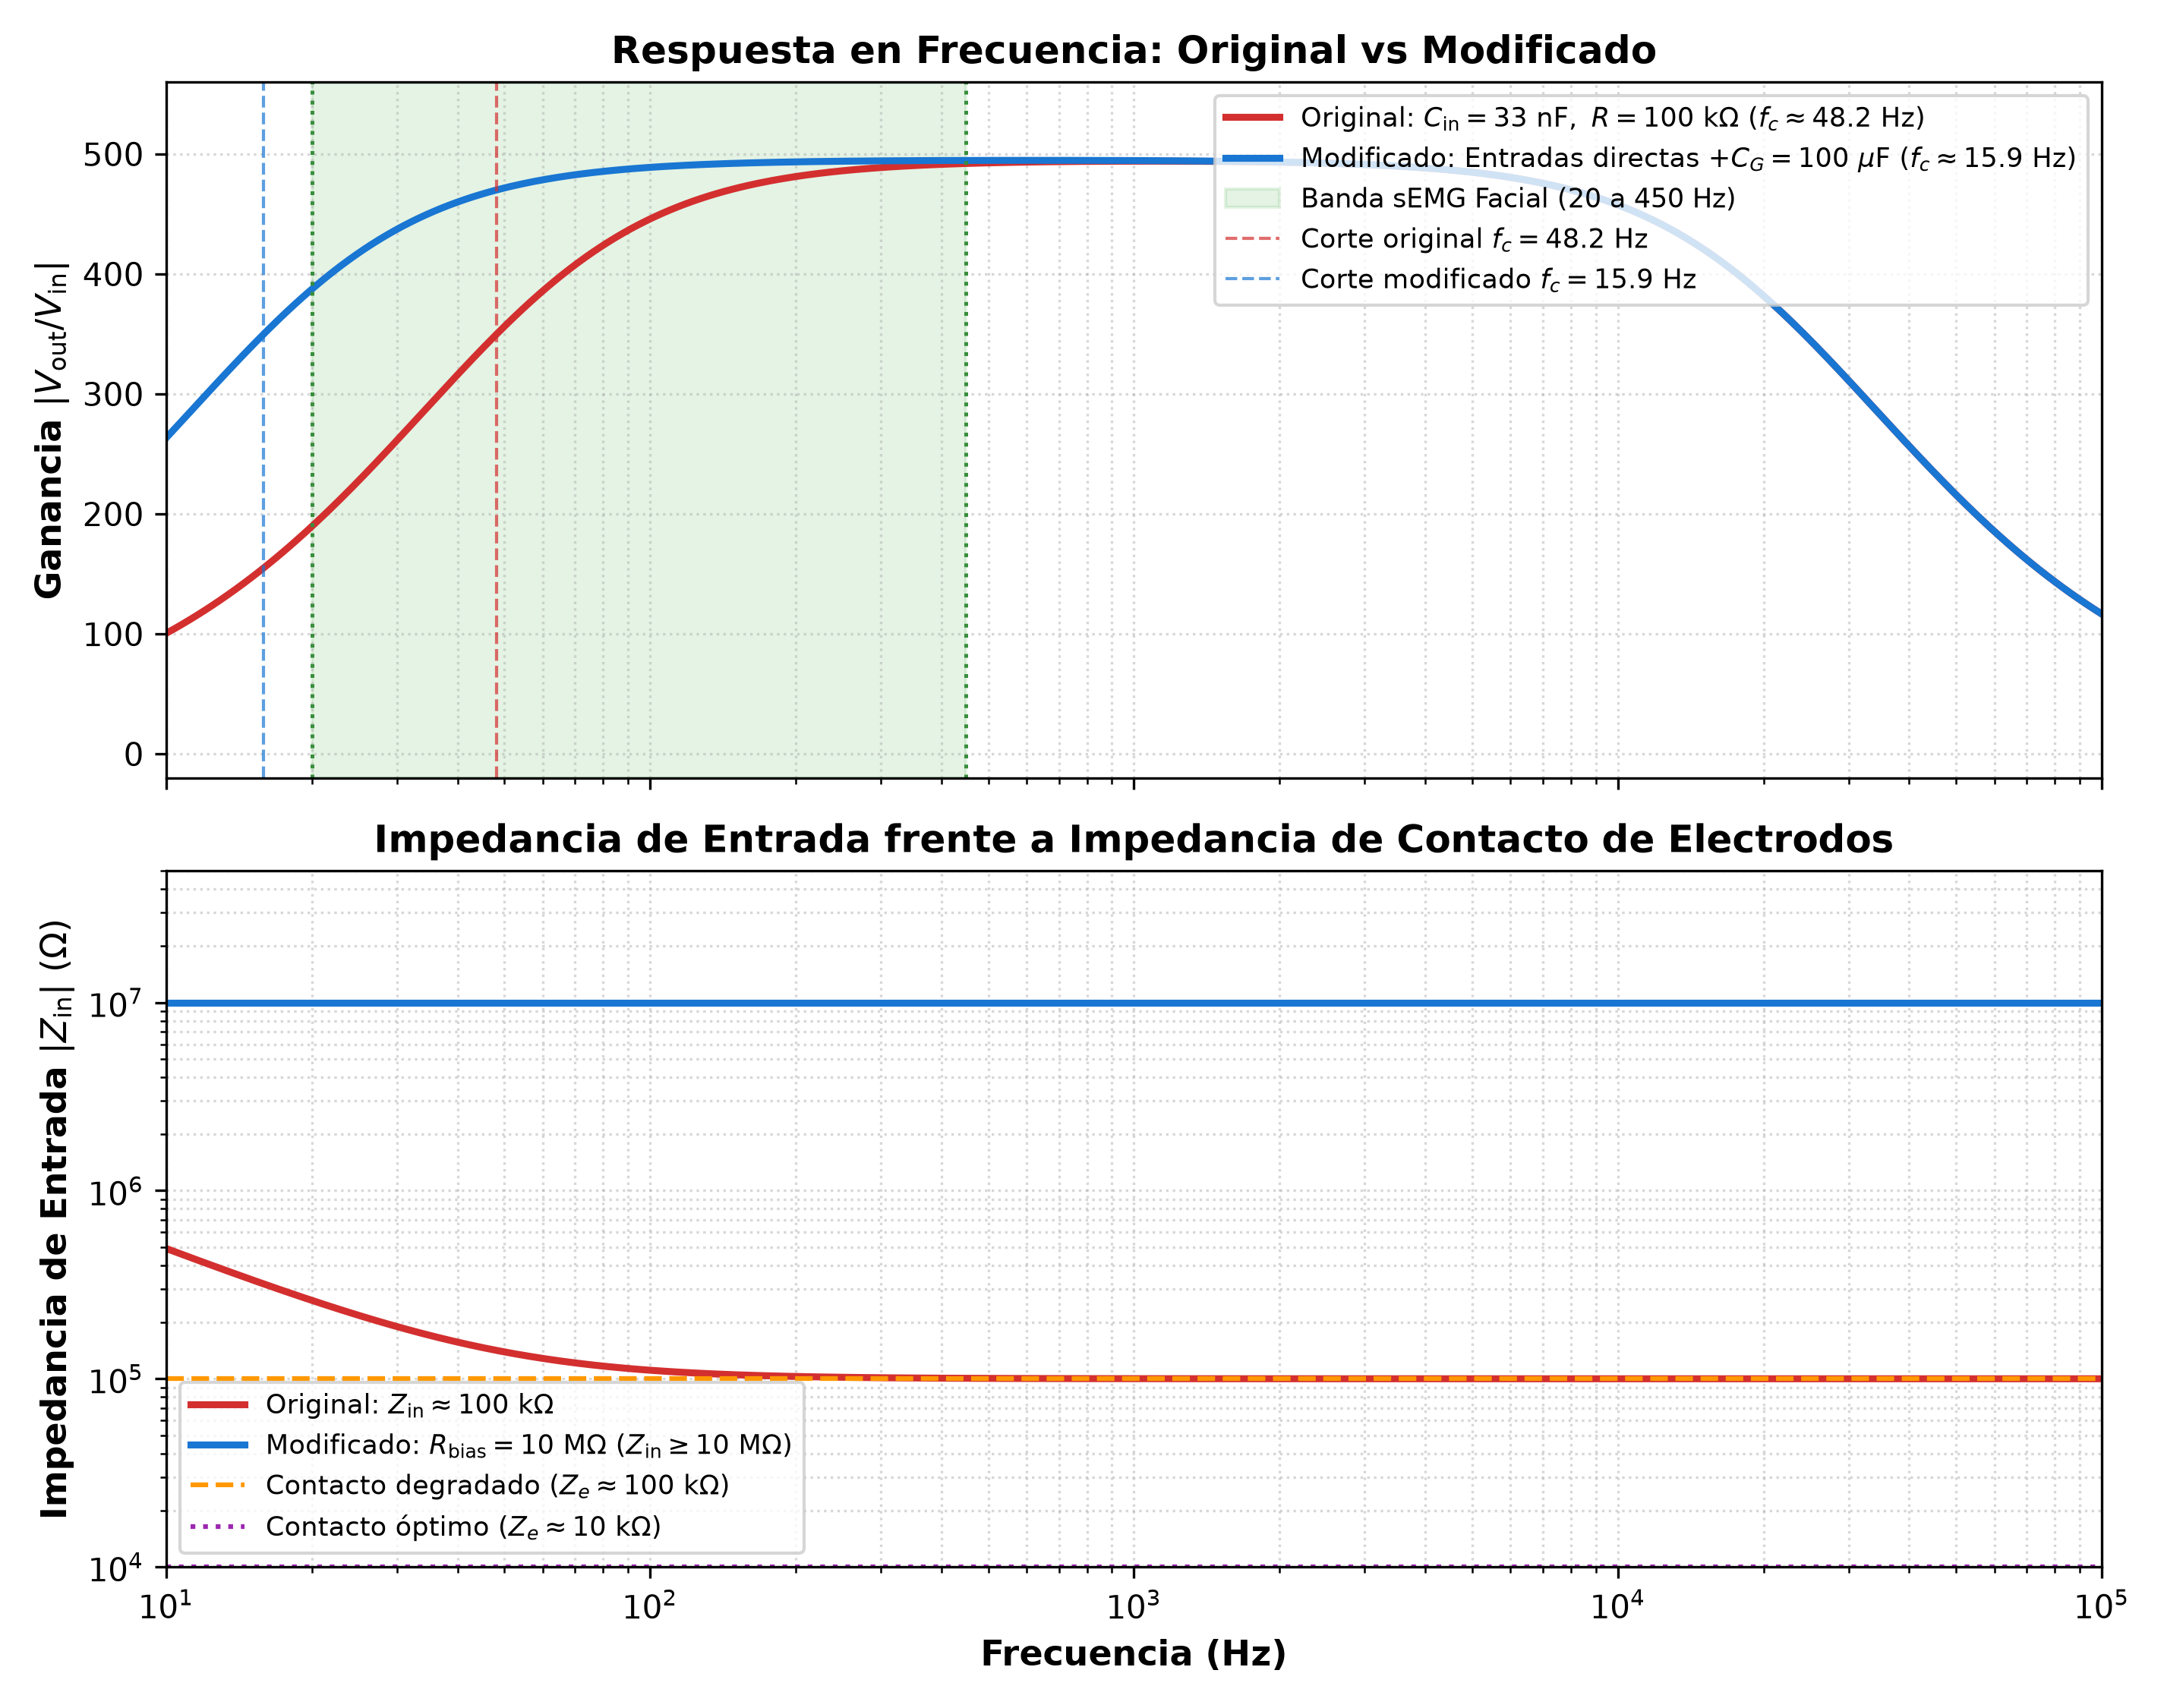
\includegraphics[width=0.88\linewidth]{imagenes/comparacion_respuesta_frecuencia_impedancia.png}
    \caption{Comparación entre el circuito actual y la modificación propuesta. Arriba: Respuesta en frecuencia destacando la recuperación de la banda sEMG facial (20 a 450 Hz) con el polo en $15.9\,\text{Hz}$. Abajo: Impedancia de entrada $Z_{\text{in}}$ frente a la impedancia de degradación del electrodo (100 k$\Omega$).}
    \label{fig:comparacion_frecuencia_impedancia}
\end{figure}

\end{document}


